\section{Results} \label{results}

\subsection{Models} \label{results:models}
Multiple models were used to evaluate the implemented methods in section \ref{implementation}. The model with the largest scale is the Disney cloud \cite{DisneyCloud}. Our implementation is bound by volumes with size $4096^3$ so we use the half resolution version. We also use multiple models from the \href{https://www.openvdb.org/download/}{OpenVDB website} and the \href{https://jangafx.com/software/embergen/download/free-vdb-animations/}{JangaFX website}. A mix of models was used with diverse axis size, number of voxels, animation frame number and shapes. 

\begin{table}[htbp]
    \centering 
    \begin{tabularx}{\textwidth}{|X|c|c|c|c|}
    \hline
    \textbf{Model} & \textbf{Voxels} & \textbf{Dimensions} & \textbf{Animation frames} & \textbf{Render}\\
    \hline
    \textbf{fire} & 4,458,790 & [160, 363, 152] & 1 & \includegraphics[width=4cm]{figures/fire.png}\\
    \hline
    \textbf{bunny} & 5,513,993 & [627, 620, 488] & 1 & \includegraphics[width=4cm]{figures/bunny.png}\\
    \hline
    \textbf{bunny cloud} & 19,210,271 & [576, 571, 437] & 1 & \includegraphics[width=4cm]{figures/bunny cloud.png}\\
    \hline
    \textbf{armadillo} & 22,734,512 & [1,275, 1,518, 1,159] & 1 & \includegraphics[width=4cm]{figures/armadilo.png}\\
    \hline
    \textbf{dragon} & 23,347,893 & [2,022, 910, 1,346] & 1 & \includegraphics[width=4cm]{figures/dragon.png}\\
    \hline
    \textbf{cloud pack} & 49,869,596 & [349, 178, 530] & 10 & \includegraphics[width=4cm]{figures/cloud pack.png}\\
    \hline
    \raggedright\textbf{disney cloud} & 188,358,293 & [993, 675, 1,224] & 1 & \includegraphics[width=4cm]{figures/disney cloud.png}\\
    \hline
    \textbf{chimney} & 239,747,485 & [160, 350, 505] & 100 & \includegraphics[width=4cm]{figures/chimney.png}\\
    \hline
    \textbf{shockwave} & 631,494,157 & [732, 140, 729] & 50 & 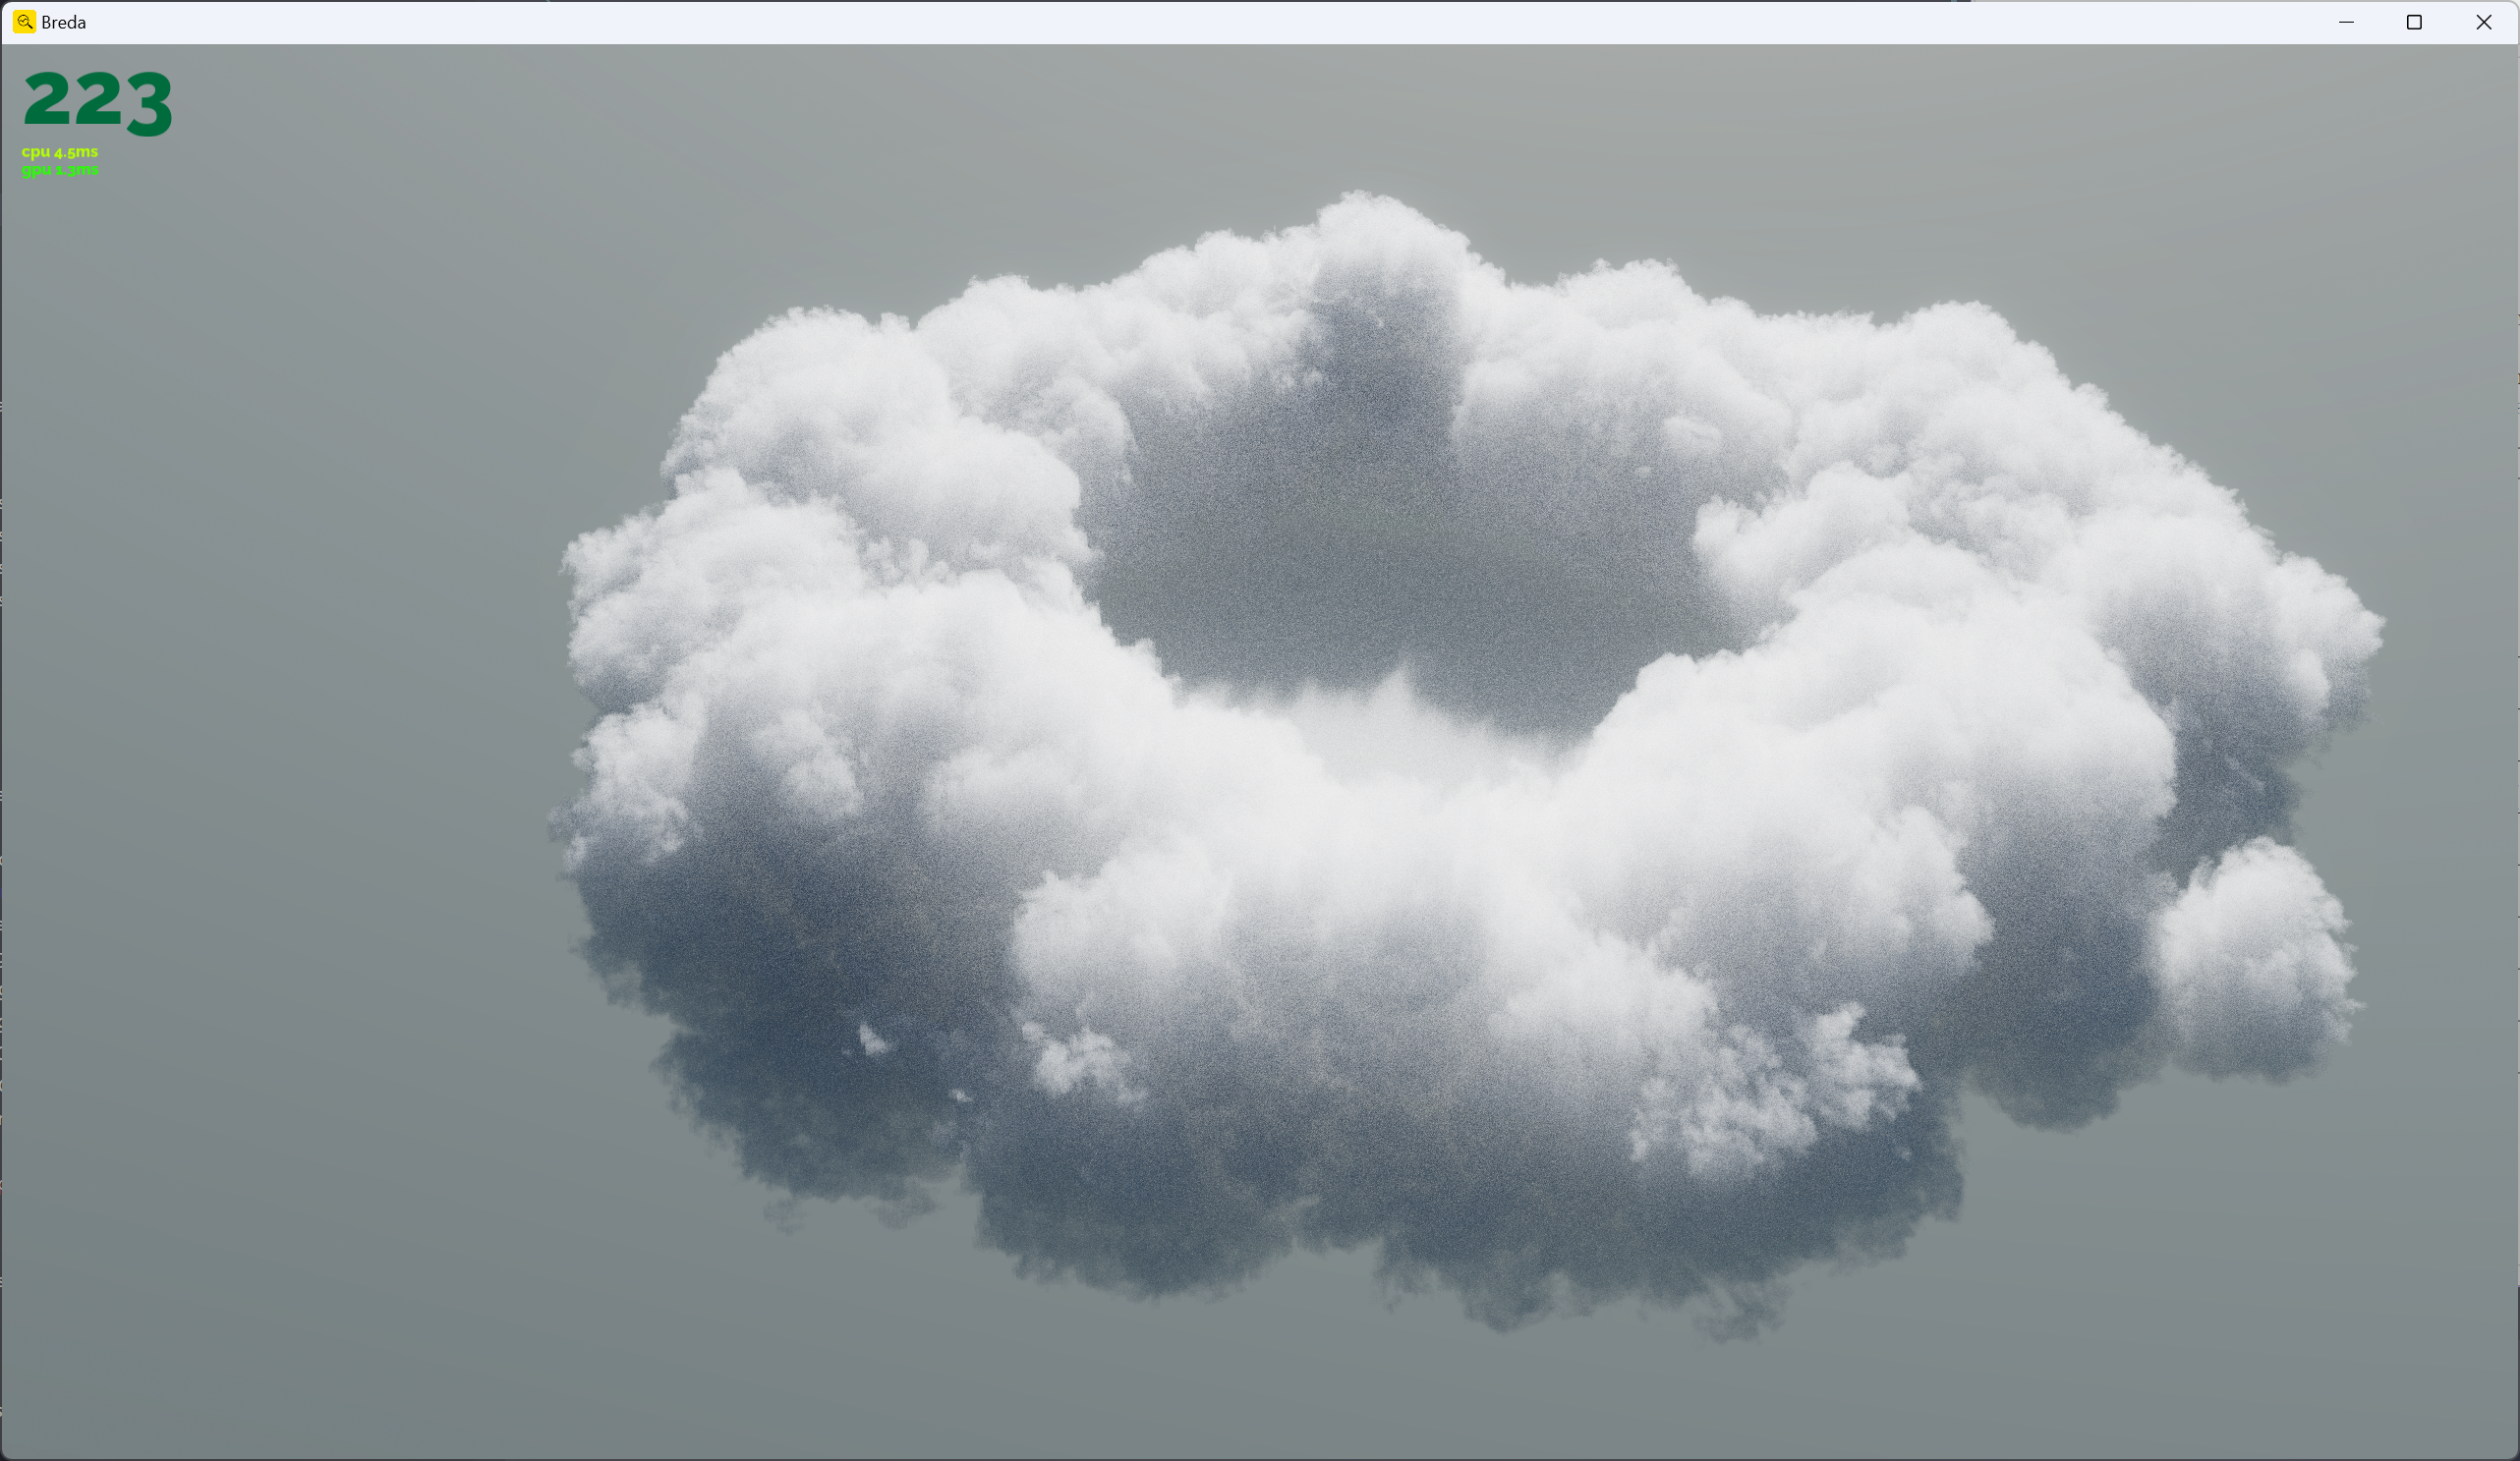
\includegraphics[width=4cm]{figures/shockwave.png}\\
    \hline
    \end{tabularx}
    \caption{The used volume models for our results. Bunny, armadillo and dragon consist of only the bounding edge of the volume. Cloud pack, chimney and shockwave contain multiple animation frames and thus can make use of delta compression. The voxels column indicates the number of non-zero voxels in the base model. All renders are done using the Breda framework using $100$ samples per pixel. }
    \label{tab:data-summary}
\end{table}


\subsection{Tree size} \label{results:tree_size}
As described in section \ref{approach:flipbook_animations}, we put our focus on compressing the voxel data instead of our tree structure size. Because of this, we did not implement any form of compression of the geometry (besides the sparse nature that already existed in VDB). This results in long animation sequences having large trees. In table \ref{tab:tree_sizes} we can see that the larger models, and animation sequences are larger than the in section \ref{requirements:asset_size} mentioned sizes. This needs to somehow be resolved, either by making our tree deeper, or deduplicating bit masks somehow. The latter would be an interesting option. We could make every node in our tree consist of two indices, one child pointer and a bitmask pointer. On one hand this would add an extra indirection to every level in our tree, but on the other, we will have many internal bit masks where every bit is true. All these nodes will thus point to the same underlying bit mask and pretty much always use cached data. The potential gains here are significant for our L3 nodes, even when all unique bit mask configurations are present. The maximum number of unique L3 nodes is $((1<<3)^3)^2 = 262,144$ which is quite a lot fewer than the number of L3 nodes present in all but one of our models. In the best case, our shockwave model, this would reduce the size of our L3 nodes by $7\times$, and again, possibly improve performance.

\begin{table}[htbp]
    \centering
    \begin{tabularx}{\textwidth}{|c|c|X|c|X|c|X|}
    \hline
    \textbf{Model} & \textbf{L1 Nodes} & \textbf{L1 size in KB} & \textbf{L2 Nodes} & \textbf{L2 size in MB} & \textbf{L3 Nodes} & \textbf{L3 size in MB} \\
    \hline
    \textbf{fire} & 1 & 4 & 32,768 & 17 & 65,536 & 4\\
    \hline
    \textbf{bunny} & 1 & 4 & 32,768 & 17 & 307,200 & 21\\
    \hline
    \textbf{bunny cloud} & 1 & 4 & 32,768 & 17 & 303,104 & 20\\
    \hline
    \textbf{armadillo} & 1 & 4 & 32,768 & 17 & 1,339,392 & 91\\
    \hline
    \textbf{dragon} & 1 & 4 & 32,768 & 17 & 1,302,528 & 88\\
    \hline
    \textbf{cloud pack} & 10 & 41 & 327,680 & 168 & 905,216 & 61\\
    \hline
    \textbf{disney cloud} & 1 & 4 & 32,768 & 17 & 1,007,616 & 69\\
    \hline
    \textbf{chimney} & 100 & 410 & 3,276,800 & 1,678 & 9,195,520 & 625\\
    \hline
    \textbf{shockwave} & 50 & 205 & 1,638,400 & 838 & 9,658,368 & 657\\
    \hline
    \end{tabularx}
    \caption{Tree sizes of the different VDB models. Each node takes exactly one 32-bit index and their bitmask in size. Which makes each L1 node 4100 bytes, each L2 node 516 bytes, and each L3 node 68 bytes. The number of L1 and L2 nodes is directly correlated with the number of animation frames as each frame has a single L1 node, and each of the children of that L1 node are allocated upfront. This makes neither the L1 nor the L2 layer sparse, but the L3 layer is sparse and thus can be smaller than the L2 layer. Its also notable how the trees do not make use of delta compression which adds a fixed cost to every animation frame, making long animations like chimney very large in memory.}
    \label{tab:tree_sizes}
\end{table}

\subsection{Block compression} \label{results:block_compression}
Block compression theoretically has a good compression ratio, by reducing our voxel data from 32 or 16 bits per voxel to 2. There are two main drawbacks of this method. Those being, (1) the reduced precision arising from the discretization into a single byte. And (2) the spatial dependency of voxel data, meaning that voxels within one brick can become inaccurate if there are outliers. We can single out the first issue by using unsigned normalized bytes (Unorm), interpolated between the minimum and maximum value of the volume. This gives us the same discretization as block compression but without the spatial dependency. For good measure we also compare against a 16-bit float per voxel version. Most VDB's are already using 16-bit floating point data which will thus not result in any difference between it and the 32-bit version. In figure \ref{fig:block_compression} we see the difference between the different data formats. Table \ref{tab:compression_rmse} shows us that all models contain a non-zero RMSE even when using the 16-bit floating point precision (although the precision difference should not be noticeable). This is due to our path tracer being non-deterministic and thus always introducing noise in all kinds of ways. However, this does not have to be an issue when we want to evaluate the accuracy of our lossy compression. Visually there is no difference for any of the models between the 32 and 16-bit formats so, we can take that as a baseline. When we have a look at the bunny and dragon models, we barely see a difference in RMSE when using different formats (the visual difference is rendered in figures \ref{fig:block_compression:bunny_bc7} and \ref{fig:block_compression:dragon_bc7}). Thus, these models work great with this compression technique. When looking at Disney cloud we see a spike when going from Unorm to BC7. This is visualized above in figure \ref{fig:block_compression:disney_unorm} (the Unorm diff) and figure \ref{fig:block_compression:disney_bc7} (the BC7 diff). There clearly are voxels which contain different values compared to their 32-bit counterpart. This likely has to do with quickly varying densities. When having a look at fire we also see a jump in error but this time when going from f16 to Unorm. When having a look at figures \ref{fig:block_compression:fire_f16} (the f16 diff) and \ref{fig:block_compression:fire_unorm} (the Unorm diff), we see that the problem lies in the top half of the model. Specifically, where the densities are very low. This can be explained by the Unorm discretization not properly capturing the subtle differences in different low density voxels. 


\clearpage
\begin{figure}[H]
    \centering
    \subfloat[]{
        \includegraphics[width=0.45\textwidth]{compare_images_pytorch/diff_disney_cloud_format_unorm.png} \label{fig:block_compression:disney_unorm}
    }
    \hfill
    \subfloat[]{
        \includegraphics[width=0.45\textwidth]{compare_images_pytorch/diff_disney_cloud_format_bc7.png} \label{fig:block_compression:disney_bc7}
    }
    \hfill
    \subfloat[]{
        \includegraphics[width=0.45\textwidth]{compare_images_pytorch/diff_fire_format_f16.png} \label{fig:block_compression:fire_f16}
    }
    \hfill
    \subfloat[]{
        \includegraphics[width=0.45\textwidth]{compare_images_pytorch/diff_fire_format_unorm.png} \label{fig:block_compression:fire_unorm}
    }
    \hfill
    \subfloat[]{
        \includegraphics[width=0.45\textwidth]{compare_images_pytorch/diff_bunny_format_bc7.png} \label{fig:block_compression:bunny_bc7}
    }
    \hfill
    \subfloat[]{
        \includegraphics[width=0.45\textwidth]{compare_images_pytorch/diff_dragon_format_bc7.png} \label{fig:block_compression:dragon_bc7}
    }
    \hfill
    \subfloat[]{

        \begin{tabular}{|l|l|l|l|}
        \hline
        \textbf{Model} & \textbf{Data Format} & \textbf{RMSE} \\
        \hline
        bunny & f16 & 0.0048 \\
        & Unorm & 0.0050 \\
        & bc7 & 0.0050 \\
        \hline
        disney cloud & f16 & 0.0089 \\
        & Unorm & 0.0089 \\
        & bc7 & 0.0135 \\
        \hline
        dragon & f16 & 0.0062 \\
        & Unorm & 0.0062 \\
        & bc7 & 0.0064 \\
        \hline
        fire & f16 & 0.0044 \\
        & Unorm & 0.0099 \\
        & bc7 & 0.0100 \\
        \hline
    \end{tabular}
    \label{tab:compression_rmse}
    }

    \caption{We compare the Root Mean Square Error (RMSE) of the compression of four different models at $1000$ samples per pixel. We calculate the difference against the full 32-bit floating point precision model as this is closest to the ground truth.} \label{fig:block_compression}
\end{figure}
\subsection{Clustering} \label{results:clustering}


\begin{figure}[H]
    \centering
    \subfloat[]{
        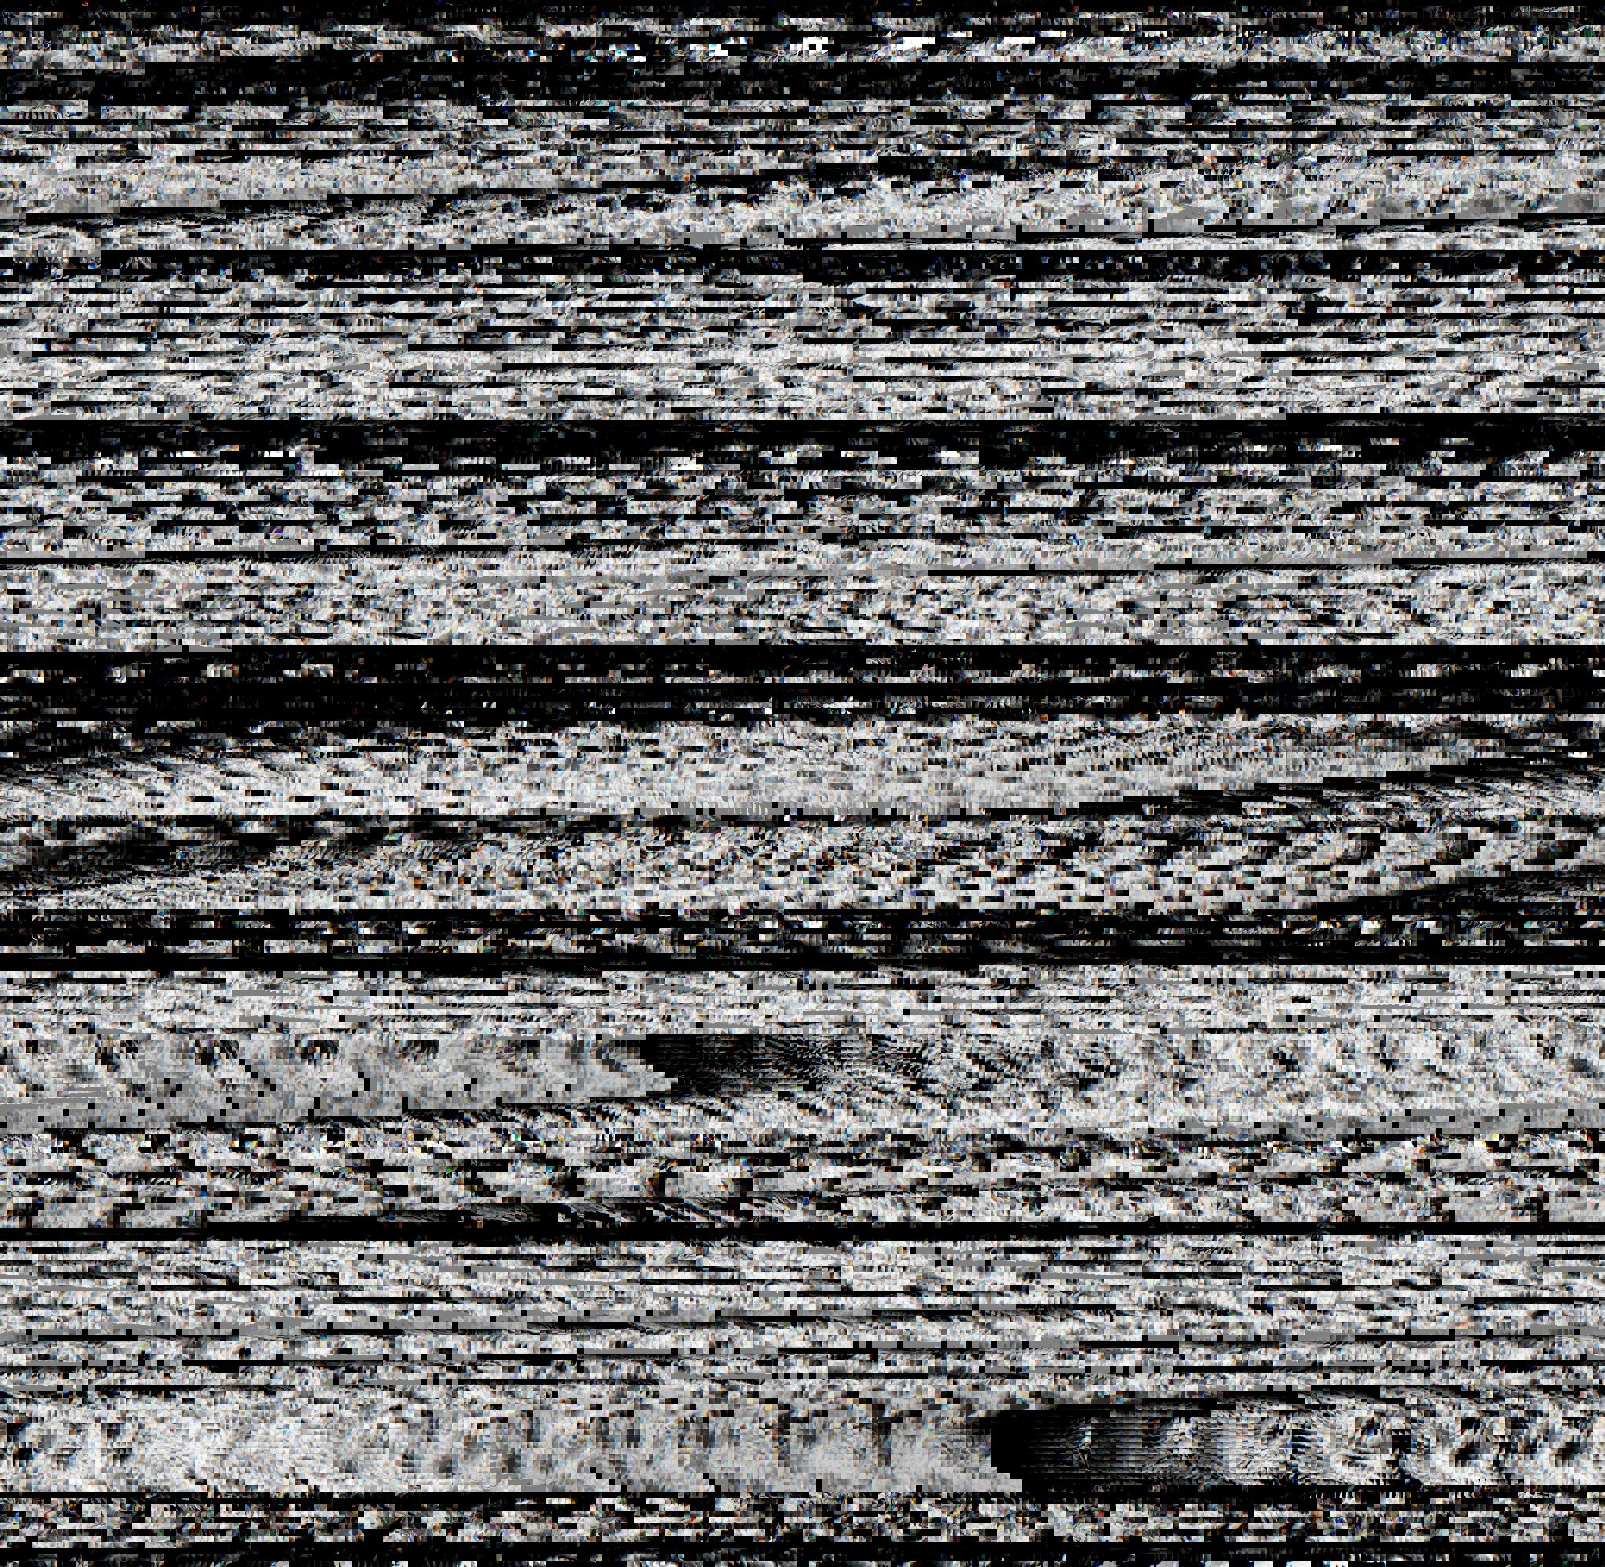
\includegraphics[width=0.45\textwidth]{figures/pre_clustered_memory.png} \label{fig:implementation:compression:pre_cluster}
    }
    \hfill
    \subfloat[]{
        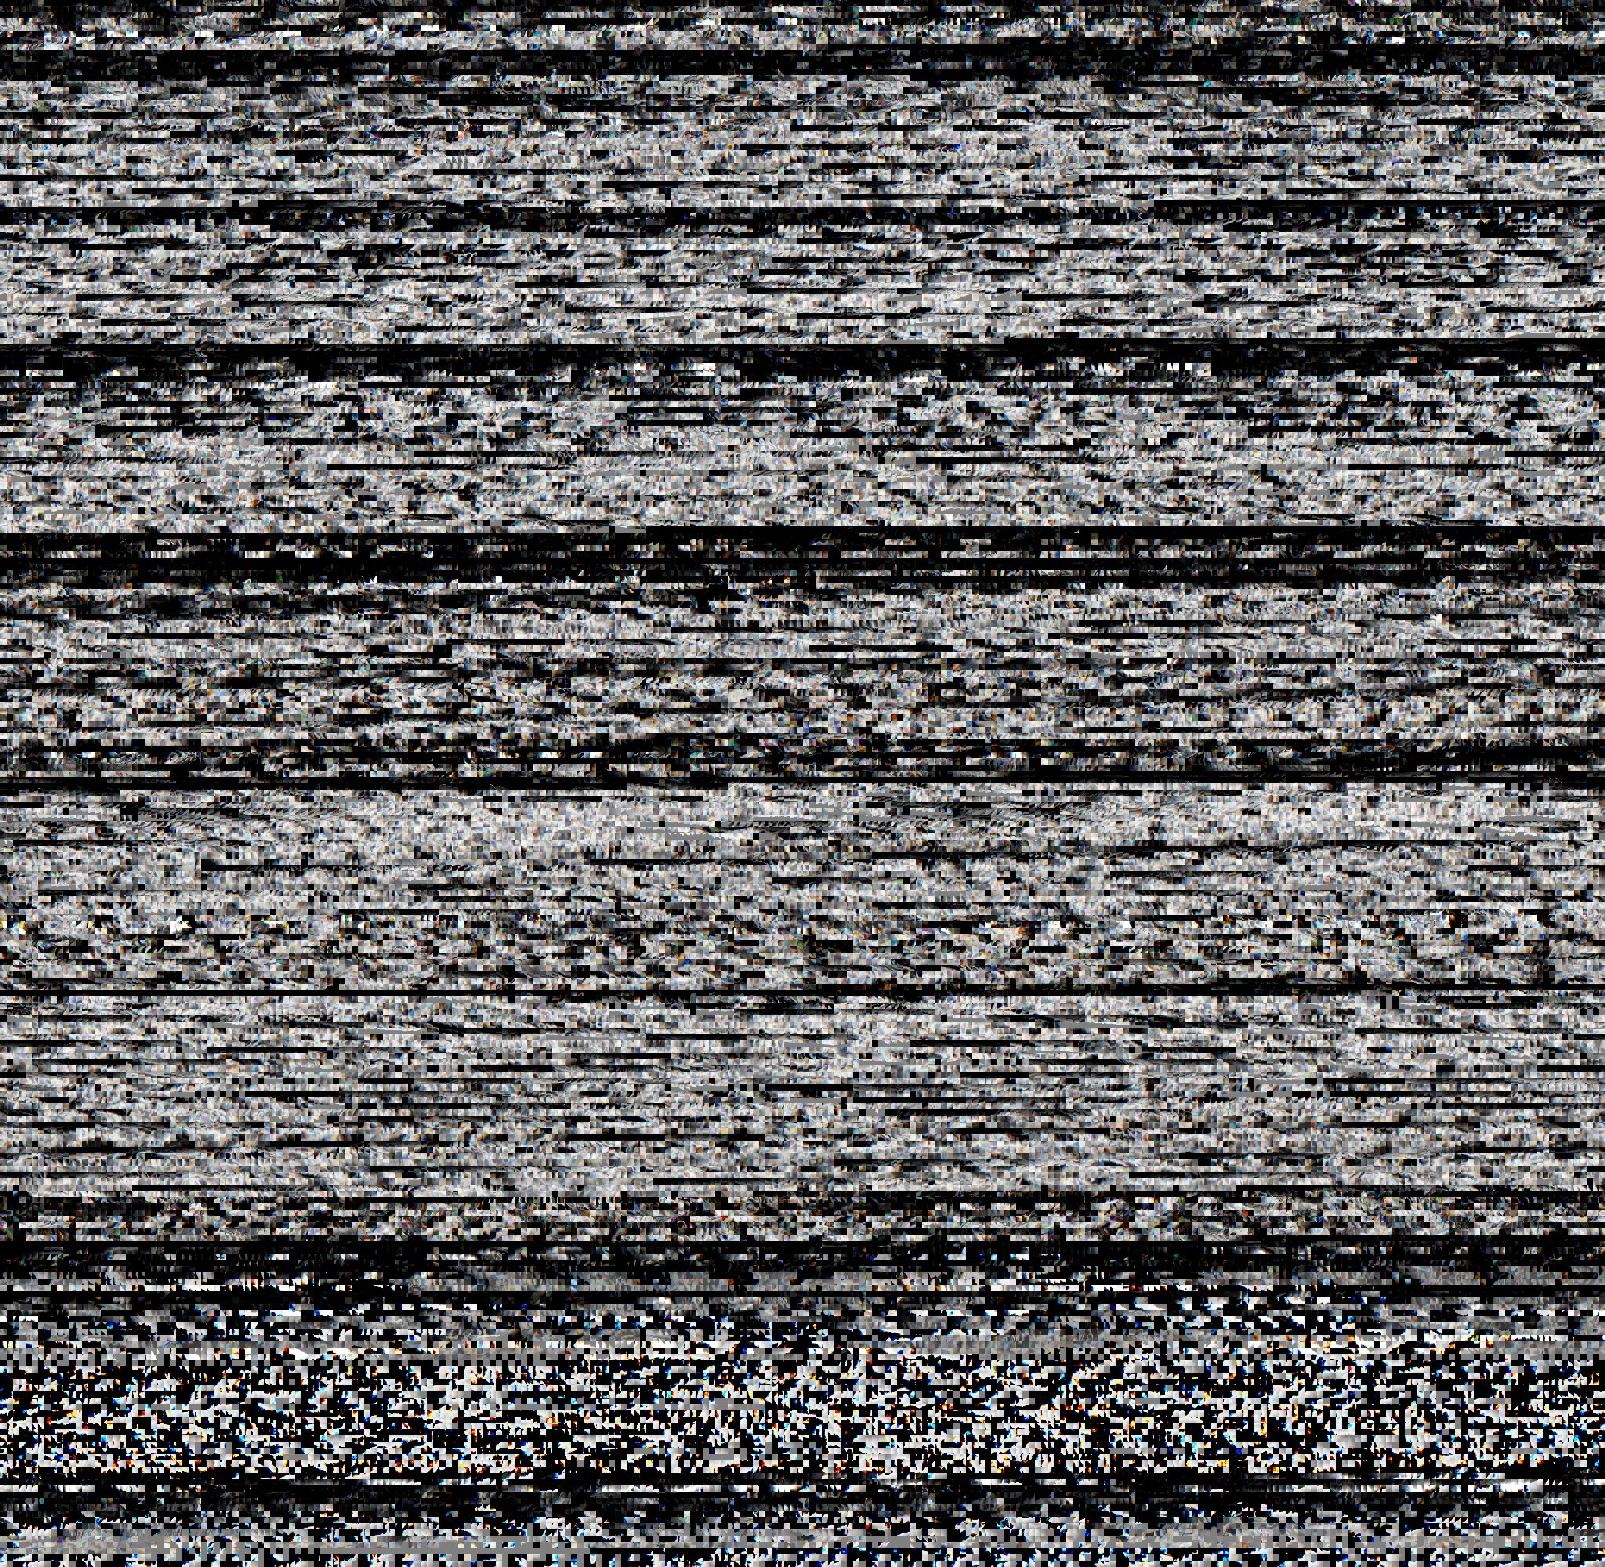
\includegraphics[width=0.45\textwidth]{figures/post_clustered_memory.png} \label{fig:implementation:compression:post_cluster}
    }
    \caption{The results of our clustering compression technique. All of these results use Bc7 encoding. Figure \ref{fig:implementation:compression:pre_cluster} shows a slice out of the voxel brick data texture on the GPU. There are visible long chains of black or otherwise greyscale slices which means that these bricks are mostly homogeneous inside that brick. In Figure \ref{fig:implementation:compression:post_cluster} we again see a slice of the voxel brick data texture, but this time after running our clustering algorithm. There are visibly fewer patches grayscale bricks when compared to figure \ref{fig:implementation:compression:pre_cluster}. This shows us that we are actually removing bricks which are homogeneous, and keeping unique nodes.} \label{fig:implementation:compression:cluster}
\end{figure}